% =====================================================================
%  Industrial Training Report -- Ishaan Singhal (23/EP/047)
%  Cadence Design Systems (India) Pvt. Ltd. -- Voltus Product Engineering
%  Compile: pdflatex report.tex  (run twice for TOC + cover border)
% =====================================================================
\documentclass[11pt,a4paper]{article}

% ---------- packages ----------
\usepackage[T1]{fontenc}
\usepackage[utf8]{inputenc}
\usepackage{mathpazo}
\usepackage[scaled=0.92]{inconsolata}
\usepackage{microtype}
\usepackage[a4paper,margin=2.3cm]{geometry}
\usepackage{graphicx}
\usepackage[table]{xcolor}
\usepackage{booktabs,tabularx,array}
\usepackage{enumitem}
\usepackage{titlesec}
\usepackage{tocloft}
\usepackage{caption}
\usepackage{float}
\usepackage{needspace}
\usepackage{listings}
\usepackage{amsmath}
\usepackage{tikz}
\usetikzlibrary{calc,positioning,arrows.meta,shapes.symbols,fit,backgrounds}
\usepackage{pgfplots}
\pgfplotsset{compat=1.17}
\usepackage{xurl}
\usepackage[hidelinks]{hyperref}

% ---------- colours ----------
\definecolor{dtublue}{RGB}{47,84,150}
\definecolor{cadred}{RGB}{200,16,46}
\definecolor{codebg}{RGB}{246,247,249}
\definecolor{rowgray}{RGB}{243,246,251}
\definecolor{okgreen}{RGB}{44,160,44}
\definecolor{outblue}{RGB}{31,119,180}
\definecolor{limorange}{RGB}{245,140,20}

% ---------- layout ----------
\linespread{1.06}
\setlength{\parskip}{4pt}
\setlength{\parindent}{0pt}
\setlist{nosep,leftmargin=1.4em,topsep=3pt}

\titleformat{\section}{\centering\LARGE\bfseries}{\thesection.}{0.4em}{}
\titlespacing*{\section}{0pt}{20pt}{16pt}
\titleformat{\subsection}{\large\bfseries}{\thesubsection}{0.6em}{}
\titlespacing*{\subsection}{0pt}{14pt}{6pt}
\titleformat{\subsubsection}{\normalsize\bfseries\color{dtublue}}{\thesubsubsection}{0.5em}{}

\renewcommand{\cftsecleader}{\cftdotfill{\cftdotsep}}
\renewcommand{\cfttoctitlefont}{\hfill\LARGE\bfseries}
\setcounter{tocdepth}{2}

\captionsetup{font=small,labelfont=bf,labelsep=colon}
\renewcommand{\arraystretch}{1.2}

\lstset{
  basicstyle=\ttfamily\footnotesize,
  backgroundcolor=\color{codebg},
  frame=single, rulecolor=\color{gray!35},
  columns=fullflexible, keepspaces=true,
  breaklines=true, framesep=6pt,
  xleftmargin=6pt, xrightmargin=6pt,
  aboveskip=8pt, belowskip=4pt,
  commentstyle=\color{gray}\itshape
}

% ---------- helpers ----------
\newcommand{\fn}[1]{\texttt{#1}}                 % file / command names
\newcommand{\dd}[2]{\textbf{#1}\newline{\small\color{gray!70!black}#2}}
\newcommand{\takeaway}[1]{\par\smallskip\noindent\textcolor{dtublue}{\textbf{Takeaway:}} #1\par}
\newcommand{\focus}[1]{\noindent\textit{Focus: #1}\par\smallskip}
\newcommand{\week}[2]{\needspace{12cm}\subsection{#1}\focus{#2}}

\newcolumntype{D}{>{\raggedright\arraybackslash}p{2.1cm}}
\newenvironment{daylog}
 {\par\noindent\rowcolors{2}{rowgray}{white}\renewcommand{\arraystretch}{1.3}%
  \tabularx{\linewidth}{@{}DX@{}}\toprule\rowcolor{white}\textbf{Day} & \textbf{Work Done}\\\midrule}
 {\bottomrule\endtabularx\par}

\tikzset{
  box/.style={draw=dtublue,rounded corners=3pt,fill=dtublue!6,align=center,
              font=\small,minimum height=1.0cm,inner sep=4pt,text width=2.7cm},
  arr/.style={-{Stealth[length=2.2mm]},thick,dtublue!80!black}
}

% =====================================================================
\begin{document}

% ---------------------------- COVER ----------------------------------
\begin{titlepage}
\begin{tikzpicture}[remember picture,overlay]
  \draw[dtublue,line width=2.2pt,rounded corners=28pt]
    ($(current page.north west)+(1.6cm,-1.6cm)$) rectangle
    ($(current page.south east)+(-1.6cm,1.6cm)$);
\end{tikzpicture}
\centering
\vspace*{1.0cm}

\includegraphics[width=4.0cm]{figures/dtu_logo.png}\par
\vspace{1.5cm}
\rule{0.8\linewidth}{1.6pt}\par\vspace{8pt}
{\Huge\textsc{Industrial Training Report}}\par\vspace{2pt}
\rule{0.8\linewidth}{1.6pt}\par
\vspace{1.3cm}
{\large Submitted in partial fulfilment for the}\par\vspace{0.5cm}
{\LARGE Degree of Bachelor of Technology,\\[4pt] Engineering Physics}\par
\vspace{1.3cm}
\textbf{Training Organisation:} Cadence Design Systems (India) Pvt.\ Ltd., Noida\\[3pt]
\textbf{Team:} Product Engineering -- Voltus (Power Integrity Signoff)\\[3pt]
\textbf{Project:} Distributed Automation for Voltus Power-Integrity Signoff\\[3pt]
\textbf{Duration:} 1 June 2026 to 31 July 2026\par
\vspace{1.4cm}
{\large\textbf{Submitted by:}}\par\vspace{6pt}
{\large\itshape ISHAAN SINGHAL\\[2pt] 23/EP/047}\par
\vfill
Department of Applied Physics, Delhi Technological University,\\
Bawana Road, Delhi-110042\par
\vspace{1.2cm}
\end{titlepage}

% ---------------------------- CONTENTS -------------------------------
\setcounter{page}{2}
\tableofcontents
\clearpage

% ======================== 1. ACKNOWLEDGEMENT =========================
\section{Acknowledgement}

I thank my \textbf{reporting manager} and the \textbf{Voltus Product Engineering team} at
Cadence Design Systems, Noida, for a second training stint with the team, for real
production problems to work on, and for fast, honest feedback on every script I shipped.

Special thanks to the teammates who reviewed my code line by line, shared legacy run
decks, and pushed each tool from ``works on my run'' to ``works on a customer database''.
I also thank the HR and IT teams for a smooth onboarding and offboarding.

I am grateful to \textbf{Delhi Technological University} for making industrial training
part of the curriculum, and to the Department of Applied Physics for the grounding in
devices, circuits and computation that this work relied on.

I acknowledge the use of AI assistants, \textbf{Claude} and \textbf{Gemini}, for drafting
and debugging code. Every suggestion was reviewed, tested on real Voltus runs and adapted by
me before use.

\vspace{1.5cm}
\begin{flushright}
\textbf{ISHAAN SINGHAL}\\
(23/EP/047)
\end{flushright}
\clearpage

% ========================= 2. INTRODUCTION ===========================
\section{Introduction}

\subsection{About the Organization}
\textbf{Cadence Design Systems} is a global leader in Electronic Design Automation (EDA).
Its software, hardware and IP are used to design and sign off integrated circuits,
systems-on-chip (SoCs) and PCBs. Flagship tools span the full flow: Virtuoso (custom/analog),
Genus (synthesis), Innovus (place \& route), Tempus (static timing) and Voltus (power
integrity). Cadence India, with major centres in Noida and Bengaluru, hosts large R\&D and
product engineering teams for these tools.

\subsection{About the Team}
The internship was with \textbf{Product Engineering (PE) -- Voltus}. Voltus is Cadence's
power-integrity signoff solution: cell-level power analysis, static and dynamic IR drop,
and electromigration (EM) on full-chip designs. The PE team sits between R\&D and customers:
\begin{itemize}
  \item validates Voltus on real and customer designs (accuracy, runtime, capacity);
  \item tunes run decks and distributed (multi-host) execution;
  \item reproduces customer issues and files minimal test cases with R\&D;
  \item builds automation around the tool's large, multi-GB report outputs.
\end{itemize}

\subsection{How the Internship was Obtained}
I had interned with the same team in June--July 2025, building a Voltus power-verification
flow and scripts to consolidate scattered missing-data reports. Based on that work, I was
taken back for a two-month industrial training in 2026.

\subsection{Internship Details}
\begin{itemize}
  \item \textbf{Organization:} Cadence Design Systems (India) Pvt.\ Ltd., Noida SEZ
  \item \textbf{Duration:} 1\textsuperscript{st} June 2026 to 31\textsuperscript{st} July 2026 (two months)
  \item \textbf{Role:} Product Engineer Intern
  \item \textbf{Mode:} On-site
  \item \textbf{Team:} Product Engineering -- Voltus (Power Integrity Signoff)
  \item \textbf{Mentor:} Reporting Manager, Voltus Product Engineering
  \item \textbf{Work:} Distributed automation for Voltus signoff reports; IR-drop ECO study
\end{itemize}

\subsection{Roles and Responsibilities}
\begin{itemize}
  \item Run and debug Voltus power and rail (IR) analysis on RAK (90\,nm) and 55\,nm designs.
  \item Tune \fn{run.tcl} settings; debug local vs.\ distributed (LSF) execution.
  \item Build distributed, multithreaded Python tools for Voltus report post-processing.
  \item Deploy and validate the tools on a customer (QCOM) database; fix LSF submission issues.
  \item Document tools (review deck, usage guide) and report tool bugs with minimal repro cases.
\end{itemize}

\subsection{Technologies Used}
\begin{center}
\begin{tabularx}{0.92\linewidth}{@{}lX@{}}
\toprule
\textbf{Area} & \textbf{Tools / Techniques}\\
\midrule
EDA tools        & Cadence Voltus (25.13), Tempus, Innovus\\
Languages        & Python 3.7, Tcl, C++ (inline, JIT-compiled at runtime), csh/bash\\
Compute          & IBM LSF (\fn{bsub}) multi-host grid, NFS shared storage, RHEL Linux\\
Parallelism      & \fn{ThreadPoolExecutor}, multiprocessing, \fn{mmap}, GNU \fn{sort --parallel}\\
Data formats     & LEF/DEF, Liberty, SPEF, TWF, VCD, \fn{.iv}, \fn{.ptiavg}, \fn{.totalcurrent}, JSON, gzip\\
Visualisation    & Matplotlib (headless Agg), Plotly\\
Docs \& workflow & GVim, NoMachine, LaTeX Beamer, PowerPoint, e-mail reviews\\
AI assistance    & Claude, Gemini (drafting, refactoring, debugging)\\
\bottomrule
\end{tabularx}
\end{center}

\subsection{Use of AI Assistance}
Claude and Gemini were used as coding assistants: drafting boilerplate (argument parsing,
logging, config loading), explaining Voltus/LSF error logs, and brainstorming edge cases.
Output was treated as a first draft. Algorithms, scheduling logic and all validation were
done by me on real Voltus data, and the final code was reviewed by teammates before hand-over.

\subsection{Background: Power Integrity in One Page}
A chip's power-grid (PG) network has finite resistance and inductance, so the supply seen by
each cell is lower than nominal. Voltus computes this drop for every instance.
\begin{align*}
  \text{Static IR:}\quad & \Delta V = I_{\text{avg}}\,R_{\text{PG}}\\
  \text{Dynamic IR:}\quad & \Delta V(t) = I(t)\,R_{\text{PG}} + L\,\frac{dI}{dt}\\
  \text{Cell power:}\quad & P = \underbrace{\alpha\,C_L V_{DD}^{2} f}_{\text{switching}}
                          + P_{\text{internal}} + \underbrace{V_{DD}\,I_{\text{leak}}}_{\text{leakage}}
\end{align*}
Voltus reports the effective voltage across each cell as
$V_{\text{DIV}} = V_{\text{PWR}} - V_{\text{GND}}$. Example from the 55\,nm design
(\fn{.iv} report, Figure~\ref{fig:iv}): $1.29176 - 0.02628 = 1.26548$\,V against a nominal
$1.32$\,V, i.e.\ an effective drop of $54.5$\,mV ($4.1\%$). The switching-activity factor
$\alpha$ is why the cell-count / switching-file cross-check (Section~\ref{sec:cellcount})
matters: a cell missing from the switching data gets the wrong power, and hence the wrong IR.

\subsection{Work Overview and Architecture}
All work orbits one fact: in distributed mode Voltus splits the chip into partitions and
writes every report per partition (\fn{part\_0/}, \fn{part\_1/}, \dots). Figure~\ref{fig:arch}
shows how the three tools I built consume these outputs.

\begin{figure}[H]
\centering
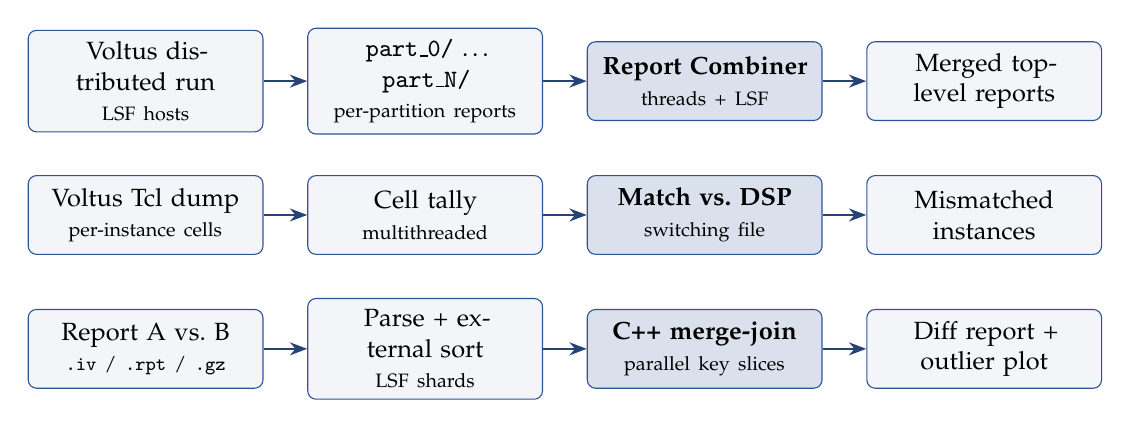
\begin{tikzpicture}
  % lane 1 : combiner
  \node[box] (v)  at (0,0)     {Voltus distributed run\\\scriptsize LSF hosts};
  \node[box] (p)  at (3.55,0)  {\fn{part\_0/} \dots\ \fn{part\_N/}\\\scriptsize per-partition reports};
  \node[box,fill=dtublue!18] (c) at (7.1,0) {\textbf{Report Combiner}\\\scriptsize threads + LSF};
  \node[box] (m)  at (10.65,0) {Merged top-level reports};
  \draw[arr] (v)--(p); \draw[arr] (p)--(c); \draw[arr] (c)--(m);
  % lane 2 : cell count
  \node[box] (t)  at (0,-1.7)     {Voltus Tcl dump\\\scriptsize per-instance cells};
  \node[box] (ct) at (3.55,-1.7)  {Cell tally\\\scriptsize multithreaded};
  \node[box,fill=dtublue!18] (cm) at (7.1,-1.7) {\textbf{Match vs.\ DSP}\\\scriptsize switching file};
  \node[box] (mm) at (10.65,-1.7) {Mismatched instances};
  \draw[arr] (t)--(ct); \draw[arr] (ct)--(cm); \draw[arr] (cm)--(mm);
  % lane 3 : comparison
  \node[box] (a)  at (0,-3.4)     {Report A vs.\ B\\\scriptsize \fn{.iv} / \fn{.rpt} / \fn{.gz}};
  \node[box] (s)  at (3.55,-3.4)  {Parse + external sort\\\scriptsize LSF shards};
  \node[box,fill=dtublue!18] (j) at (7.1,-3.4) {\textbf{C++ merge-join}\\\scriptsize parallel key slices};
  \node[box] (o)  at (10.65,-3.4) {Diff report +\\outlier plot};
  \draw[arr] (a)--(s); \draw[arr] (s)--(j); \draw[arr] (j)--(o);
\end{tikzpicture}
\caption{The three automation tools built around Voltus distributed outputs}
\label{fig:arch}
\end{figure}

\begin{center}
\begin{tabularx}{\linewidth}{@{}clX@{}}
\toprule
\textbf{\#} & \textbf{Deliverable} & \textbf{Key techniques}\\
\midrule
1 & Distributed Voltus Report Combiner & LPT load balancing, LSF dispatch, thread pools, C++ \fn{mmap} k-way merge\\
2 & Cell-Count / DSP Cross-Check       & Tcl instance dump, multithreaded chunked parsing, set matching\\
3 & Distributed Comparison Utility     & composite keys, external sort, parallel C++ merge-join, outlier plots\\
4 & Voltus--Tempus--Innovus ECO Study  & IR hotspot extraction, STA, physical ECO, post-ECO recheck\\
5 & Voltus Merge-Bug Report            & data-integrity check, minimal reproducible case\\
\bottomrule
\end{tabularx}
\end{center}
\clearpage

% ===================== 3. INTERNSHIP CERTIFICATE =====================
\section{Internship Certificate}
\begin{center}
\setlength{\fboxsep}{0pt}\setlength{\fboxrule}{0.4pt}
\fcolorbox{gray!40}{white}{
\includegraphics[width=0.84\linewidth]{figures/certificate.pdf}}
\end{center}
\clearpage

% ======================== 4. MONTHLY REPORTS =========================
\section{Monthly Reports}

\subsection*{First Month (June, 2026)}
Onboarding, Voltus fundamentals and the first two production scripts. After setting up the
VM and tool environment, I ran static IR analysis on the 90\,nm RAK and the 55\,nm
\textit{racerunner} design, then debugged why distributed runs stayed on local CPUs and why
rail analysis failed only in distributed mode. The second half went into scripting.

\textbf{Major tasks:}
\begin{itemize}
  \item VM, tool and LSF environment setup; study of legacy run decks.
  \item Static IR runs (90\,nm RAK, 55\,nm racerunner); \fn{run.tcl} runtime tuning.
  \item Local vs.\ distributed debug: power analysis OK in both, rail analysis fails distributed.
  \item Missing-report combiner (multithreaded + LSF), later extended to all report types.
  \item Cell-count / DSP switching cross-check: built, reviewed, re-targeted to a new run,
        made distributed, edge-case bug fixed.
  \item Kick-off of a self-driven Voltus--Tempus--Innovus ECO study.
\end{itemize}
\textbf{Outcome:} Two working, reviewed scripts that turn hour-scale Voltus post-processing
into minutes, plus a solid feel for the Voltus signoff flow.

\subsection*{Second Month (July, 2026)}
Review, deployment and hardening. The month opened with a manager-requested review of all
scripts (PPT + final code by mail), continued with the ECO study in Innovus, and then moved
to deploying the comparison utility on a customer (QCOM) database, where LSF submission bugs
were fixed and an outlier-plotting module was added and proven on customer data.

\textbf{Major tasks:}
\begin{itemize}
  \item Script review deck and final code submission (1--3 July).
  \item Innovus ECO on IR hotspots, new DEF, Voltus re-run and before/after comparison.
  \item QCOM deployment: \fn{bsub} command fixes, requirement gaps closed.
  \item Outlier plot module (relative/absolute bounds, top-N worst) proven on QCOM data.
  \item Found and documented a Voltus instance-power merge inconsistency for R\&D.
  \item Combiner usage guide, hand-over, laptop return and offboarding.
\end{itemize}
\textbf{Outcome:} Tools running on customer-scale data with documentation, one tool bug
reported upstream, and a complete hand-over to the team.
\clearpage

% ========================= 5. WEEKLY REPORTS =========================
\section{Weekly Reports}

% ------------------------------ WEEK 1 -------------------------------
\week{Week 1 (1 June to 5 June 2026)}{Onboarding and environment setup}
\begin{daylog}
\dd{Monday}{01-06-2026} & Joined Cadence, Noida. Laptop issued; HR/IT onboarding and document
signing (NDA, policies). Raised access requests for Linux compute, LSF farm and project disk.\\
\dd{Tuesday}{02-06-2026} & Manager briefing on the team charter and upcoming work. Started
Linux VM setup; remote desktop through NoMachine.\\
\dd{Wednesday}{03-06-2026} & VM bring-up continued: shell environment, tool paths for
Voltus/Tempus/Innovus, license variables, scratch and project directories. Short 8-ball pool
break with the team.\\
\dd{Thursday}{04-06-2026} & Received legacy scripts and run decks from earlier work. Laptop
and VM setup completed; tool-launch sanity checks passed.\\
\dd{Friday}{05-06-2026} & Walked through the legacy scripts; read Voltus basics (power
analysis modes, static vs.\ dynamic IR, EM). Next week assigned: RAK walkthrough and first
static IR run.\\
\end{daylog}
\takeaway{a clean, reproducible environment is the first deliverable in EDA work.}

% ------------------------------ WEEK 2 -------------------------------
\week{Week 2 (8 June to 12 June 2026)}{Voltus hands-on and distributed-run debugging}
\begin{daylog}
\dd{Monday}{08-06-2026} & Received Voltus \fn{.tcl} run decks. Studied the RAK (Rapid Adoption
Kit) static IR flow: design import (LEF/DEF, Liberty, SPEF) $\rightarrow$ power analysis
$\rightarrow$ rail analysis $\rightarrow$ reports.\\
\dd{Tuesday}{09-06-2026} & First static IR run on the 90\,nm RAK design; read power reports
and IR-drop maps.\\
\dd{Wednesday}{10-06-2026} & Static analysis on the 55\,nm \textit{racerunner} design
($\approx$6.47\,M instances, 1.32\,V nominal, multiple HV/LV rails). Noted runtime and
memory scaling vs.\ 90\,nm.\\
\dd{Thursday}{11-06-2026} & Teammate sync: cut runtime by tuning power-analysis mode
settings in \fn{run.tcl}. Manager sync: root-cause why jobs stayed
on local CPUs and why the distributed-host (LSF) setup was not taking effect.\\
\dd{Friday}{12-06-2026} & Presented results: power analysis passes local and distributed
(distributed clearly faster); rail analysis fails only in distributed mode, passes locally.
Assigned two scripting tasks.\\
\end{daylog}
\takeaway{isolate failures per stage (power vs.\ rail) before blaming the grid.}

% ------------------------------ WEEK 3 -------------------------------
\week{Week 3 (15 June to 19 June 2026)}{Missing-report combiner and cell-count script}
\begin{daylog}
\dd{Monday}{15-06-2026} & Started the ``missing-file'' script: gather missing-data reports
(\fn{power.missingdata.*}, missing-instance/cell lists) scattered across \fn{part\_*}
folders and merge them in one pass, bypassing Voltus' slow sequential merge.\\
\dd{Tuesday}{16-06-2026} & Added thread-pool multithreading and LSF (\fn{bsub}) distribution;
tuned per feedback and mailed the manager. Started the second script. Quick win at the pool
table.\\
\dd{Wednesday}{17-06-2026} & Cell-count script: dump per-instance cell data from Voltus (Tcl),
tally cell counts, match against the dynamic switching file from DSP generation. Prototype
demo to a teammate; feedback noted.\\
\dd{Thursday}{18-06-2026} & Implemented the teammate's changes. Multithreaded chunked reader:
millions of lines parsed and dumped in seconds.\\
\dd{Friday}{19-06-2026} & Asked to modify the config for a new Voltus run and re-run the
script on its output. Config parameters due Monday; prepared the run area and reviewed the
parsing logic.\\
\end{daylog}
\takeaway{parallel I/O plus de-duplication turns hour-scale merges into minutes.}

% ------------------------------ WEEK 4 -------------------------------
\week{Week 4 (22 June to 26 June 2026)}{Validation on a new run, distribution and hardening}
\begin{daylog}
\dd{Monday}{22-06-2026} & Created the new config, fired the Voltus run and demoed the script.
Team flagged output inconsistent with the new run's report structure.\\
\dd{Tuesday}{23-06-2026} & Fixed the parser for the new format; revised script validated on
the run. New request: an extra column in the final report for readability.\\
\dd{Wednesday}{24-06-2026} & Made the script distributed (LSF shards) on top of
multithreading, with per-shard logs and a final merge step.\\
\dd{Thursday}{25-06-2026} & Found and fixed an edge-case bug during testing; script stable.
Waiting for the column specification.\\
\dd{Friday}{26-06-2026} & No task assigned. Planned a self-driven Voltus $\rightarrow$ Tempus
$\rightarrow$ Innovus ECO study to see the full power/timing signoff loop.\\
\end{daylog}
\takeaway{scripts must survive format changes between runs; re-test on every new run.}

% ------------------------------ WEEK 5 -------------------------------
\week{Week 5 (29 June to 3 July 2026)}{ECO study kick-off and script review deck}
\begin{daylog}
\dd{Monday}{29-06-2026} & Baseline Voltus run for the ECO study: IR-drop maps, worst-instance
list, hotspot regions.\\
\dd{Tuesday}{30-06-2026} & Tempus STA on the same design: no setup/hold violations, so IR
fixes could proceed without timing risk.\\
\dd{Wednesday}{01-07-2026} & Manager requested a review of all scripts: final code plus
working explained in a PPT, by mail. Started code review and clean-up.\\
\dd{Thursday}{02-07-2026} & Built the deck: problem, architecture, config, usage and logs for
the combiner and cell-count scripts; runtime gains from multithreading + distribution.\\
\dd{Friday}{03-07-2026} & Final pass; mailed the PPT and final scripts to the manager.\\
\end{daylog}
\takeaway{explaining code to others forces a cleaner architecture.}

% ------------------------------ WEEK 6 -------------------------------
\week{Week 6 (6 July to 10 July 2026)}{Innovus ECO and post-ECO recheck}
\begin{daylog}
\dd{Monday}{06-07-2026} & Imported the design into Innovus. ECO on IR hotspots (PG
reinforcement, decap insertion, cell spreading); exported the modified DEF.\\
\dd{Tuesday}{07-07-2026} & Voltus re-run on the ECO DEF; before/after IR comparison showed the
localized hotspots reduced.\\
\dd{Wednesday}{08-07-2026} & Set up a Tempus recheck on the post-ECO database. Noted
trade-offs: decap area vs.\ leakage, cell spreading vs.\ wirelength.\\
\dd{Thursday}{09-07-2026} & Wrote flow notes; cleaned run directories and logs to free disk
quota. End-of-week pool session with the team.\\
\dd{Friday}{10-07-2026} & \textbf{Refresh Day} -- company-wide day off.\\
\end{daylog}
\takeaway{an IR fix is a physical change; every ECO needs a power and a timing recheck.}

% ------------------------------ WEEK 7 -------------------------------
\week{Week 7 (13 July to 17 July 2026)}{Deployment on the customer (QCOM) database}
\begin{daylog}
\dd{Monday}{13-07-2026} & New assignment: validate the comparison script (and, in parallel,
the combiner) on the QCOM customer database of \fn{.iv} signoff reports.\\
\dd{Tuesday}{14-07-2026} & First runs: parsing fine, but LSF job submission failed with
\fn{bsub} command errors under the customer farm settings. Debugged submission strings and
shard logs.\\
\dd{Wednesday}{15-07-2026} & Fixed \fn{bsub} command construction (queue, resource-string
formatting, memory and host span); shards dispatched correctly. Combiner tweaks in parallel.\\
\dd{Thursday}{16-07-2026} & Runs completed, but not all requirements were met. New task: plot
the outliers of the comparison and prove it on QCOM data.\\
\dd{Friday}{17-07-2026} & Defined the outlier rule (relative \% and absolute limits) and top-N
worst extraction; started streaming extraction from the comparison report.\\
\end{daylog}
\takeaway{customer environments expose assumptions hidden in local runs.}

% ------------------------------ WEEK 8 -------------------------------
\week{Week 8 (20 July to 24 July 2026)}{Outlier plotting and proof on QCOM data}
\begin{daylog}
\dd{Monday}{20-07-2026} & Built the plot module: Value-1 vs.\ Value-2 scatter, $y=x$
reference, $\pm r\%$ / $\pm a$ limit lines, outliers highlighted; headless Matplotlib (Agg)
PNG at 250\,dpi.\\
\dd{Tuesday}{21-07-2026} & Tested locally on a racerunner \fn{.iv} pair ($\approx$6.47\,M
instances); tuned marker size/alpha for millions of points; bounded min-heap for top-N.\\
\dd{Wednesday}{22-07-2026} & Hooked the plot into all execution paths (local, grid,
low-memory); ran on the QCOM database through LSF.\\
\dd{Thursday}{23-07-2026} & Cross-checked plotted outliers against raw rows; submitted plots
and scripts to the manager.\\
\dd{Friday}{24-07-2026} & Validated combiner output against Voltus' own merged
\fn{power.instpwr.rpt.gz}: found instance-level mismatches between partition and top-level
values.\\
\end{daylog}
\takeaway{a plot is proof only when every point traces back to a raw row.}

% ------------------------------ WEEK 9 -------------------------------
\week{Week 9 (27 July to 31 July 2026)}{Bug report, documentation and hand-over}
\begin{daylog}
\dd{Monday}{27-07-2026} & Root-caused the mismatch to Voltus' own merge, not the script:
one decap instance shows 7.578e-14 in \fn{part\_0} but 4.198e-14 at top level. Built a
minimal reproducible case.\\
\dd{Tuesday}{28-07-2026} & Prepared the bug deck for the tool team: Voltus 25.13-s099\_1, run
script, \fn{zgrep} evidence (Section~\ref{sec:bug}).\\
\dd{Wednesday}{29-07-2026} & Wrote the combiner ``Usage and Output Guide'' (Beamer): run
commands, config, outputs, logs, sample run.\\
\dd{Thursday}{30-07-2026} & Final clean-up; handed over scripts, configs and guides; closing
review with the manager.\\
\dd{Friday}{31-07-2026} & Last day: backed up work to the team area, returned the laptop to IT,
completed HR offboarding. Farewell game of pool.\\
\end{daylog}
\takeaway{a bug report is only as good as its smallest reproducible case.}
\clearpage

% ===================== 6. TECHNICAL DELIVERABLES =====================
\section{Technical Deliverables}

\subsection{Design Under Analysis}
Most runs used the 55\,nm \textit{racerunner} design. Key numbers, read directly from
Voltus outputs (Figures~\ref{fig:pwr} and \ref{fig:iv}):

\begin{minipage}[c]{0.44\linewidth}
\small
\begin{tabular}{@{}ll@{}}
\toprule
Instances       & 6,470,422\\
Nominal supply  & 1.32\,V (\fn{VDD\_LV\_COR})\\
Total power     & 3832.6\,mW\\
\quad Internal  & 45.94\%\\
\quad Switching & 41.69\%\\
\quad Leakage   & 12.37\%\\
Partitions      & 3 (\fn{part\_0}--\fn{part\_2})\\
\bottomrule
\end{tabular}
\end{minipage}\hfill
\begin{minipage}[c]{0.54\linewidth}
\centering
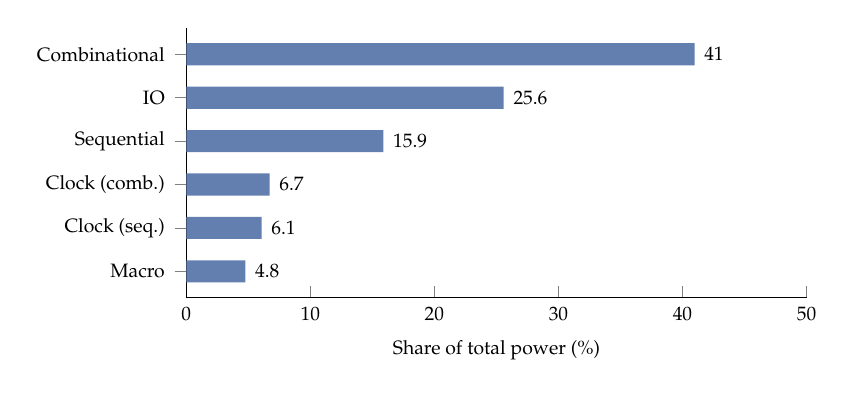
\begin{tikzpicture}
\begin{axis}[
  xbar, width=0.78\linewidth, height=5.0cm, bar width=8pt,
  xmin=0, xmax=50, ytick={1,...,6},
  yticklabels={Macro,Clock (seq.),Clock (comb.),Sequential,IO,Combinational},
  tick label style={font=\scriptsize}, label style={font=\scriptsize},
  xlabel={Share of total power (\%)},
  axis x line*=bottom, axis y line*=left, enlarge y limits=0.12,
  point meta=x,
  nodes near coords={\pgfmathprintnumber[fixed,precision=1]{\pgfplotspointmeta}},
  every node near coord/.append style={font=\scriptsize}]
\addplot[fill=dtublue!75,draw=none] coordinates
  {(4.764,1) (6.065,2) (6.709,3) (15.89,4) (25.59,5) (40.97,6)};
\end{axis}
\end{tikzpicture}
\end{minipage}

\begin{figure}[H]
\centering
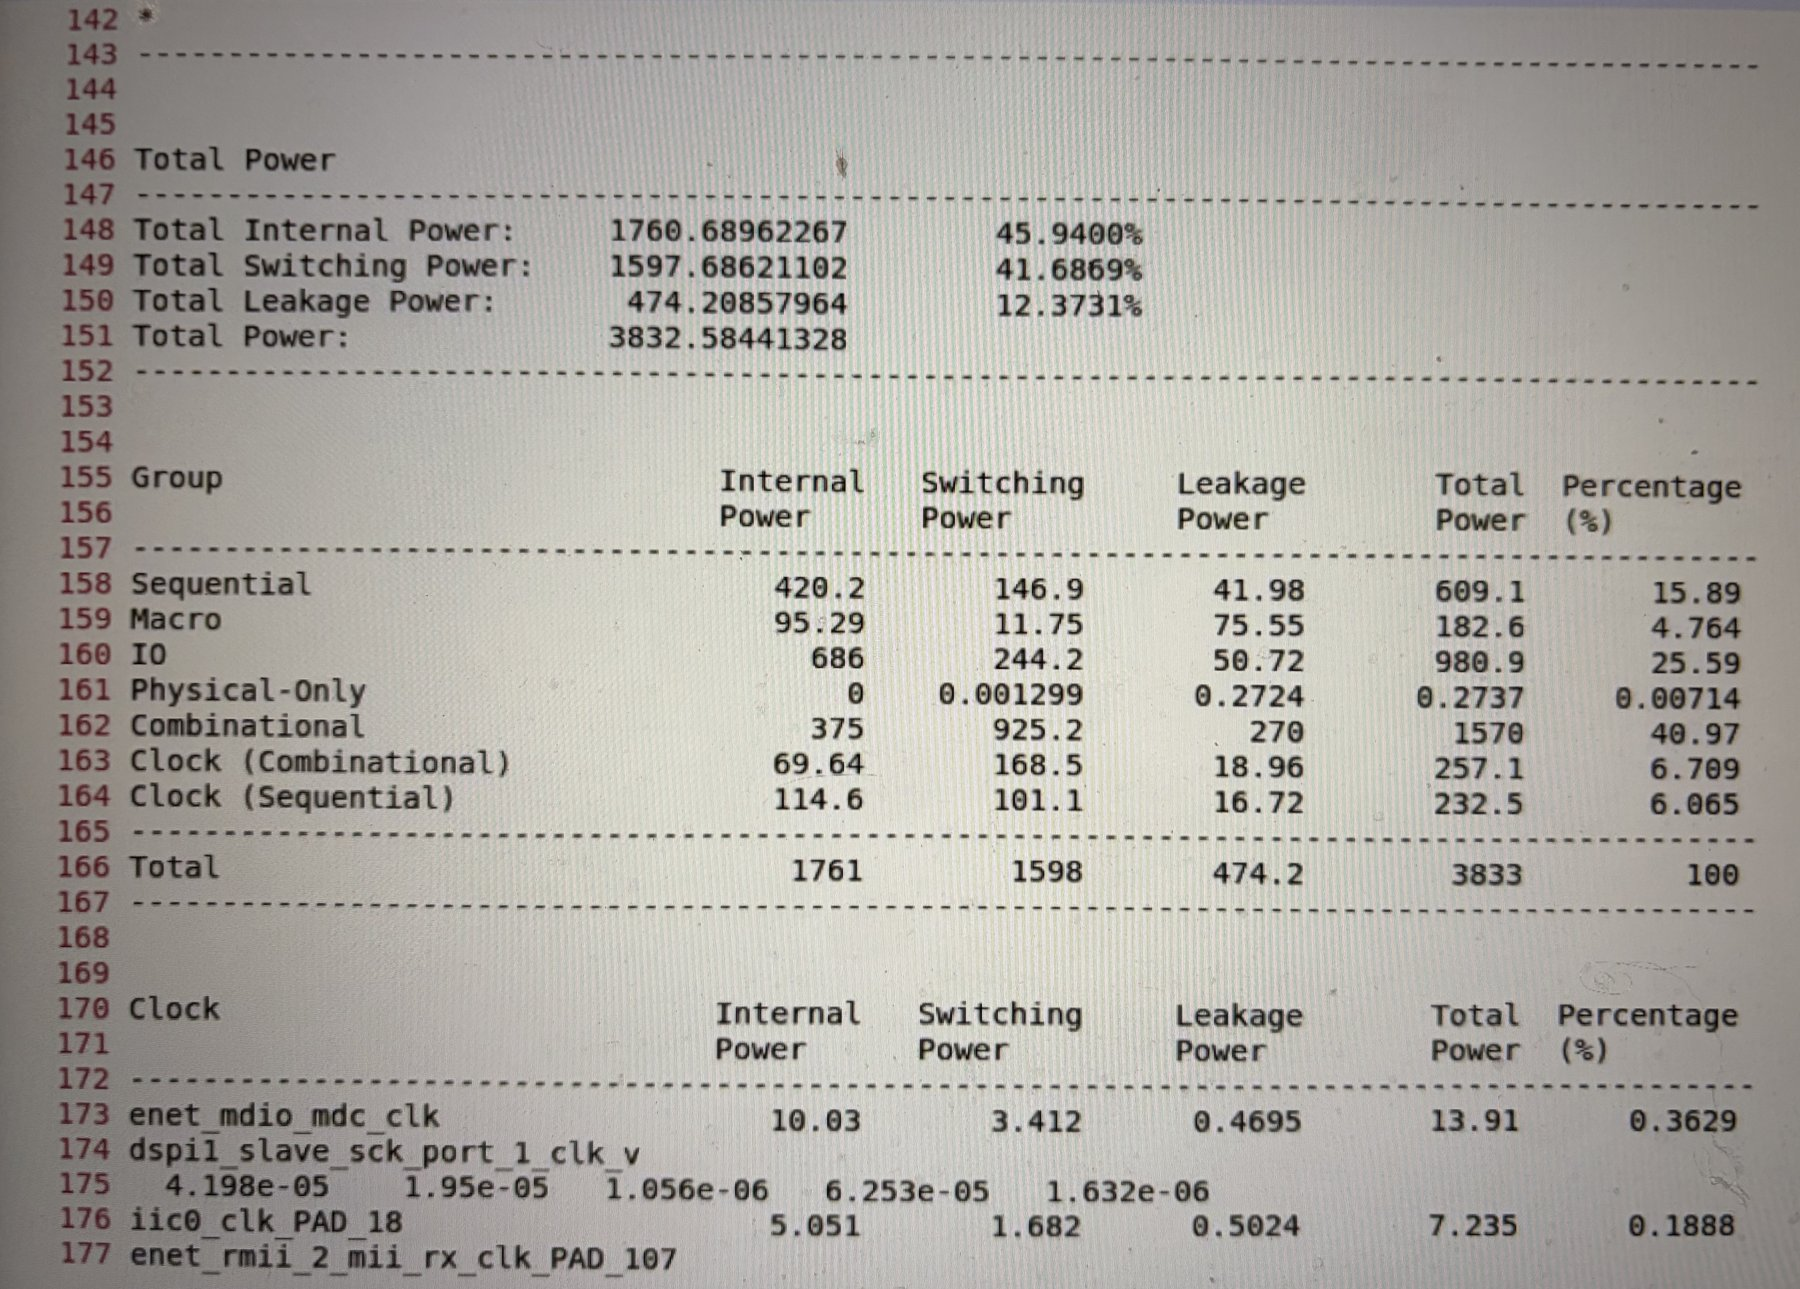
\includegraphics[width=0.72\linewidth]{figures/photo_power_rpt.jpg}
\caption{Voltus power report of racerunner: total and per-group internal, switching and leakage power}
\label{fig:pwr}
\end{figure}

% ------------------------------------------------------------------
\subsection{Distributed Voltus Report Combiner}
\textbf{Problem.} A distributed Voltus run leaves 100+ report types split across
\fn{part\_*} folders (Figure~\ref{fig:parts}). Voltus' own merge is sequential and can take up
to an hour. \textbf{Goal:} rebuild every top-level report in minutes.

\begin{figure}[H]
\centering
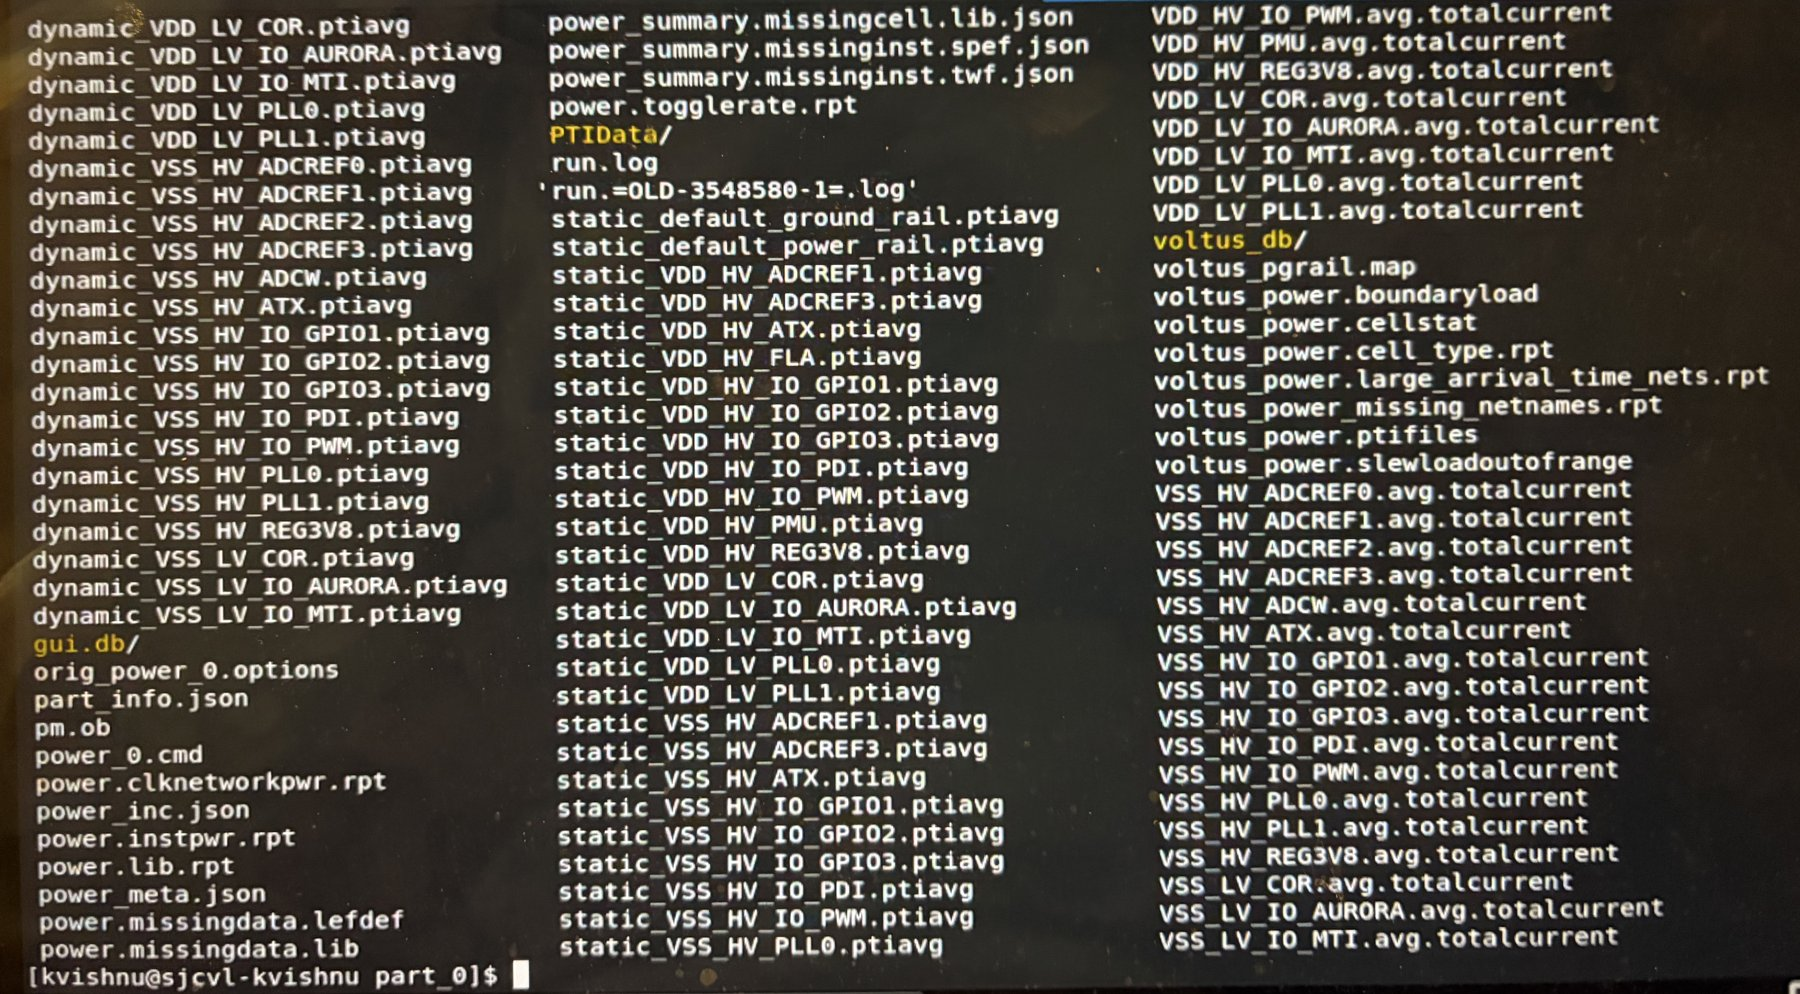
\includegraphics[width=0.8\linewidth]{figures/photo_partition.jpg}
\caption{Contents of one partition folder (\fn{part\_0/}): power, IR (\fn{.ptiavg}),
current waveforms (\fn{.totalcurrent}), JSON stats and missing-data reports}
\label{fig:parts}
\end{figure}

\begin{figure}[H]
\centering
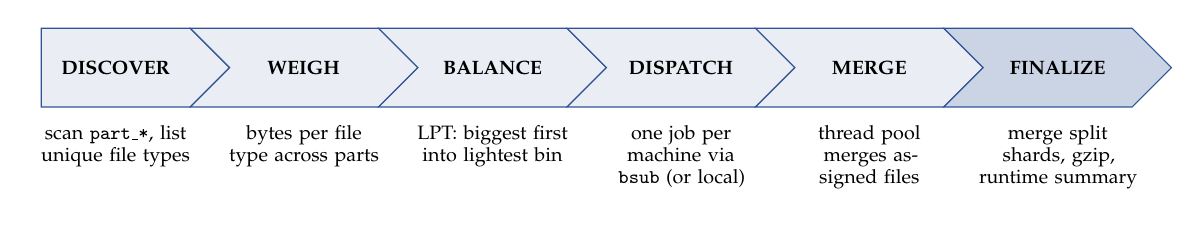
\begin{tikzpicture}[
  chev/.style={signal,signal to=east,signal from=west,draw=dtublue,fill=dtublue!10,
               minimum height=1.0cm,text width=1.75cm,align=center,
               font=\scriptsize\bfseries,inner sep=2pt},
  note/.style={text width=2.0cm,align=center,font=\scriptsize}]
  \node[chev,signal from=nowhere] (s1) {DISCOVER};
  \node[chev,right=-0.5pt of s1] (s2) {WEIGH};
  \node[chev,right=-0.5pt of s2] (s3) {BALANCE};
  \node[chev,right=-0.5pt of s3] (s4) {DISPATCH};
  \node[chev,right=-0.5pt of s4] (s5) {MERGE};
  \node[chev,right=-0.5pt of s5,fill=dtublue!25] (s6) {FINALIZE};
  \node[note,below=3pt of s1] {scan \fn{part\_*}, list unique file types};
  \node[note,below=3pt of s2] {bytes per file type across parts};
  \node[note,below=3pt of s3] {LPT: biggest first into lightest bin};
  \node[note,below=3pt of s4] {one job per machine via \fn{bsub} (or local)};
  \node[note,below=3pt of s5] {thread pool merges assigned files};
  \node[note,below=3pt of s6] {merge split shards, gzip, runtime summary};
\end{tikzpicture}
\caption{Combiner pipeline}
\label{fig:combflow}
\end{figure}

\textbf{Merge strategy per file type} (routed automatically by file name):
\begin{center}
\small
\begin{tabularx}{\linewidth}{@{}lX@{}}
\toprule
\textbf{File type} & \textbf{Merge rule}\\
\midrule
\fn{*.totalcurrent}               & sum current per aligned time step (waveforms)\\
\fn{*.json} (stats)               & recursive dictionary merge, numeric counters summed\\
missing-inst / missing-cell JSON  & streaming, disk-backed de-dup of [instance, cell] pairs (no OOM)\\
\fn{power.instpwr / power.rpt}    & structured merge; ``Total Power'' blocks re-summed\\
\fn{power.pgnet.detailed.rpt.gz}  & grouped by rail; SI-unit parse/format; chip totals recomputed\\
other \fn{.gz} and text           & \fn{sort -u --parallel} de-dup + C++ \fn{mmap} k-way merge\\
\bottomrule
\end{tabularx}
\end{center}

\textbf{Scheduling knobs.}
\begin{itemize}
  \item \textbf{Auto-local:} input below \fn{auto\_local\_gb} (5\,GB) runs locally; grid queue
        overhead would be slower.
  \item \textbf{Profiles:} \fn{light} / \fn{heavy} LSF profiles pick cores, memory and shard count
        by input size.
  \item \textbf{Heavy-file split:} files above \fn{heavy\_split\_gb} are prepared per partition in
        parallel, then merged in a finalize phase.
  \item \textbf{Observability:} \fn{master.log} + \fn{worker\_N.log} in a hidden \fn{.work\_files/}
        folder.
\end{itemize}

\needspace{7.5cm}
\begin{lstlisting}[caption={Trimmed \texttt{combine.cfg}}]
[combine]
search_dir = <run>/reports/power            # parent of part_* folders
out_dir    = <run>/reports/power/combined
grid       = 1                              # 1 = LSF farm, 0 = local

[default]
auto_local_gb = 5.0

[profile:light]
max_gb = 40.0
shard_count = 4
cores = 8
finalize_cores = 16
bsub_base_cmd = bsub -q lnx64 -W 120 -R "rusage[mem=64000] span[hosts=1]"
\end{lstlisting}

\textbf{Result on a real run} (from the runtime summary, Figure~\ref{fig:comblog}):
\begin{center}
\small
\begin{tabular}{@{}ll@{}}
\toprule
Partitions / unique file types & 3 / 115\\
Total input                    & 1.951\,GB\\
Workers                        & 4 (96 local threads each)\\
Fastest / slowest worker       & 11.3\,s / 197.6\,s\\
\textbf{Total wall time}        & \textbf{3\,min 17\,s} (vs.\ up to $\sim$1\,h sequential)\\
\bottomrule
\end{tabular}
\end{center}

\begin{figure}[H]
\centering
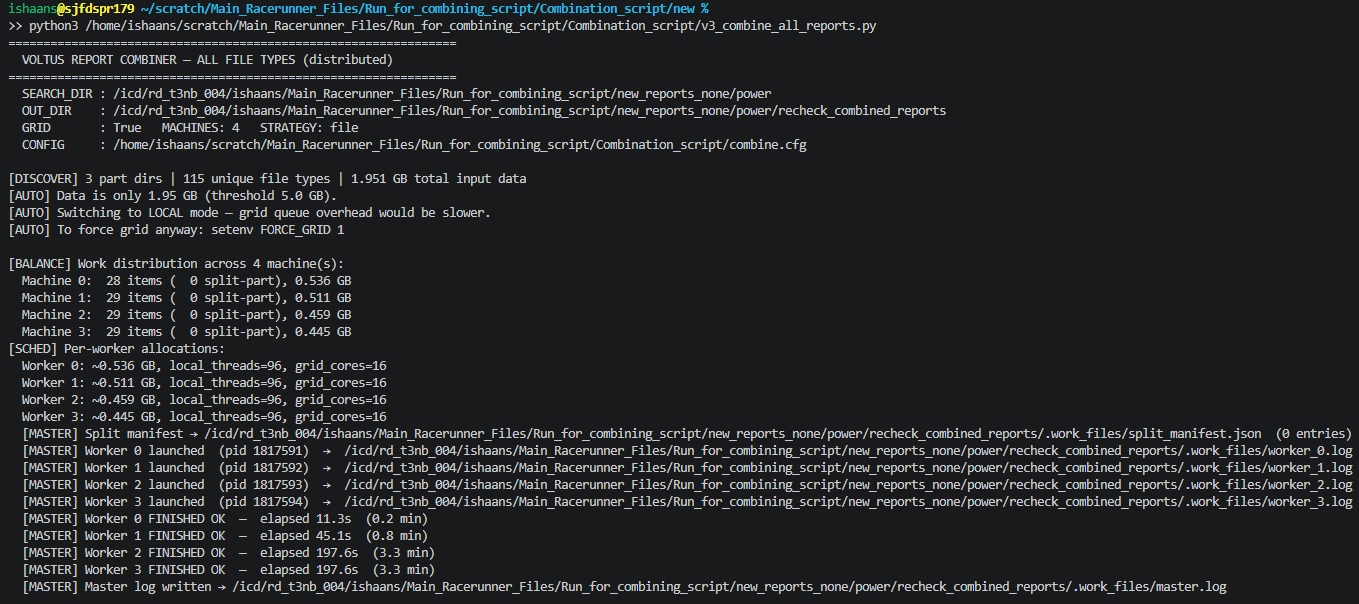
\includegraphics[width=\linewidth]{figures/combiner_log.png}\\[4pt]
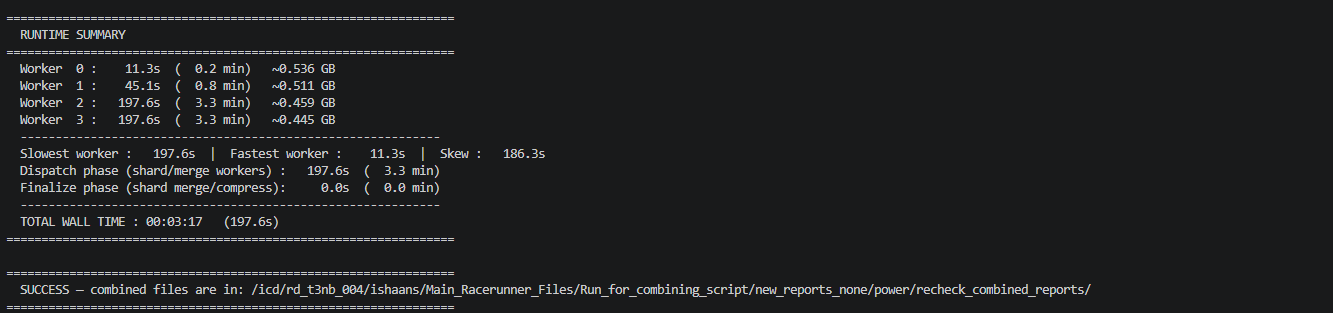
\includegraphics[width=\linewidth]{figures/combiner_runtime.png}
\caption{Combiner run: discovery, auto-local decision, load balance across 4 workers, runtime summary}
\label{fig:comblog}
\end{figure}

\begin{figure}[H]
\centering
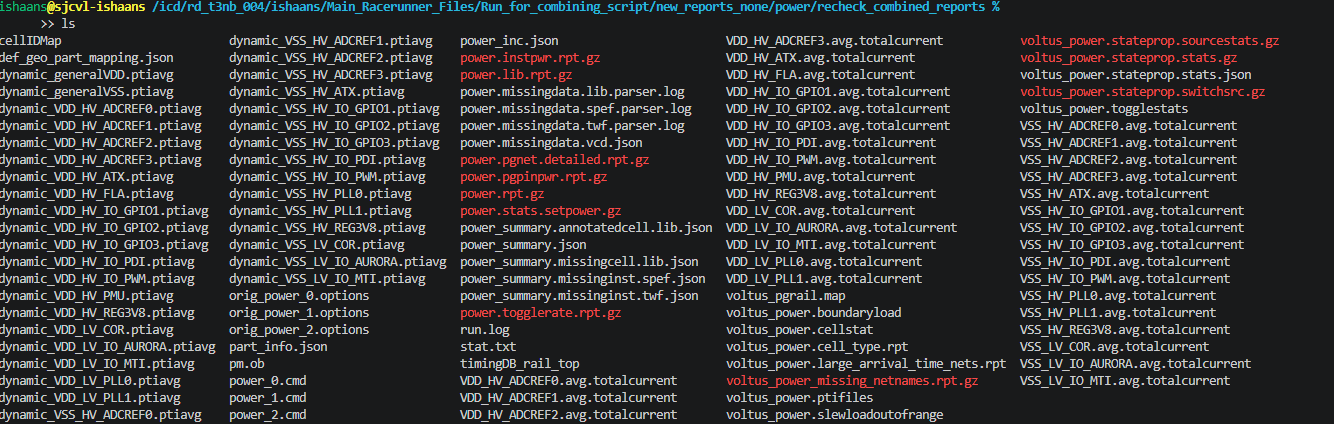
\includegraphics[width=\linewidth]{figures/combiner_output.png}
\caption{Consolidated top-level output directory produced by the combiner}
\end{figure}

% ------------------------------------------------------------------
\subsection{Cell-Count / DSP Switching Cross-Check}
\label{sec:cellcount}
\textbf{Problem.} Every instance must appear in the dynamic switching file produced during DSP
generation; a missing or extra instance silently skews switching power ($\alpha$) and IR.
\textbf{Approach:}
\begin{itemize}
  \item Tcl: tuned DSP/power-analysis settings; dump per-instance cell data from Voltus.
  \item Python: multithreaded chunked reader; tally cell counts per cell type.
  \item Match against the switching file; flag missing, extra and count-mismatched instances.
  \item Re-targeted to a new run config (Week 4), made LSF-distributed, edge case fixed.
\end{itemize}
\textbf{Outcome:} a one-command coverage check that reads and dumps millions of lines in
seconds; an extra readability column was requested and left pending spec at hand-over.

% ------------------------------------------------------------------
\subsection{Distributed Comparison Utility with Outlier Plotting}
\textbf{Problem.} Compare two signoff reports instance by instance (e.g.\ two \fn{.iv} IR
reports, each $\approx$6.47\,M lines, Figure~\ref{fig:size}) and show where and how much they
differ. Scale target: billion-row inputs on a customer database.

\begin{figure}[H]
\centering
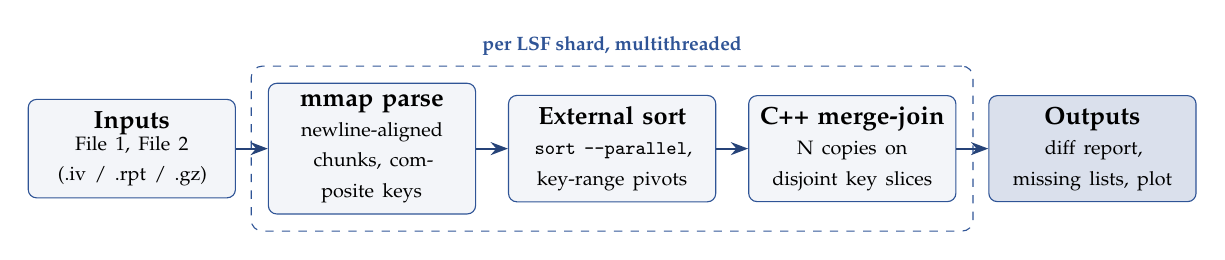
\begin{tikzpicture}[b/.style={box,text width=2.35cm,minimum height=1.25cm}]
  \node[b] (i) at (0,0)      {\textbf{Inputs}\\\scriptsize File 1, File 2\\(.iv / .rpt / .gz)};
  \node[b] (p) at (3.05,0)   {\textbf{mmap parse}\\\scriptsize newline-aligned chunks, composite keys};
  \node[b] (s) at (6.1,0)    {\textbf{External sort}\\\scriptsize \fn{sort --parallel}, key-range pivots};
  \node[b] (j) at (9.15,0)   {\textbf{C++ merge-join}\\\scriptsize N copies on disjoint key slices};
  \node[b,fill=dtublue!18] (o) at (12.2,0) {\textbf{Outputs}\\\scriptsize diff report, missing lists, plot};
  \draw[arr] (i)--(p); \draw[arr] (p)--(s); \draw[arr] (s)--(j); \draw[arr] (j)--(o);
  \begin{scope}[on background layer]
    \node[draw=dtublue,dashed,rounded corners=4pt,fit=(p)(s)(j),inner sep=6pt,
          label={[font=\scriptsize\bfseries,text=dtublue]above:{per LSF shard, multithreaded}}] {};
  \end{scope}
\end{tikzpicture}
\caption{Comparison pipeline}
\end{figure}

\textbf{Key features.}
\begin{itemize}
  \item Any column pair: user selects instance column(s) and value column per file;
        composite keys like \fn{0,2}; plain or gzip input.
  \item Output row: \fn{Instance | Value1 | Value2 | Diff | Dev\%}, plus instances missing
        on either side.
  \item LSF sharding by \fn{gb\_per\_shard}; \fn{light}/\fn{heavy} profiles; low-memory mode
        on by default.
  \item Inline C++ merge-join compiled at runtime, run in parallel on key-range slices, so the
        finalize step uses all allocated cores.
\end{itemize}

\needspace{3.5cm}
\begin{lstlisting}[caption={Typical invocation (IR comparison of two runs)}]
python3 comparison_script_distributed.py \
    --file1 runA/VDD_LV_COR_VSS_LV_COR.avg.iv --instcol1 1 --valcol1 2 \
    --file2 runB/VDD_LV_COR_VSS_LV_COR.avg.iv --instcol2 1 --valcol2 2 \
    -r 5 -a 0.01 -n 100 --outdir cmp_out
\end{lstlisting}

\textbf{Outlier rule.} For each matched instance with values $v_1, v_2$:
\[
  \text{diff} = v_1 - v_2,\qquad
  \text{dev} = \frac{v_1 - v_2}{v_2}\times 100\%,\qquad
  \text{outlier} \iff |\text{dev}| > r \;\lor\; |\text{diff}| > a .
\]
The $N$ worst rows are kept in a bounded min-heap ($O(M\log N)$ for $M$ rows) and written
to a summary; all points are drawn in one static PNG (Figure~\ref{fig:outlier}).

\begin{figure}[H]
\centering
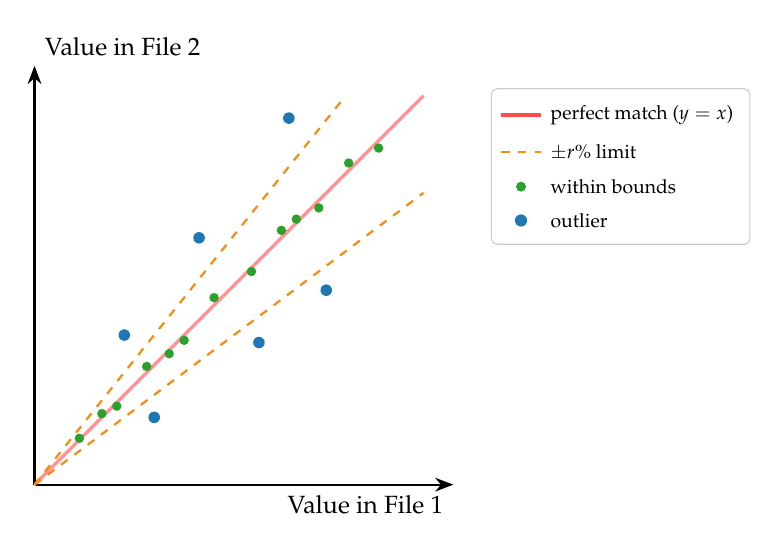
\begin{tikzpicture}[scale=0.95]
  \draw[-{Stealth},thick] (0,0) -- (5.6,0) node[below left,font=\small] {Value in File 1};
  \draw[-{Stealth},thick] (0,0) -- (0,5.6) node[above right,font=\small] {Value in File 2};
  \draw[red!70,line width=1.2pt,opacity=0.6] (0,0) -- (5.2,5.2);
  \draw[limorange,dashed,thick] (0,0) -- (4.16,5.2);
  \draw[limorange,dashed,thick] (0,0) -- (5.2,3.9);
  \foreach \x/\y in {0.6/0.62,0.9/0.95,1.1/1.05,1.5/1.58,1.8/1.75,2.0/1.93,2.4/2.5,
                     2.9/2.85,3.3/3.4,3.5/3.55,3.8/3.7,4.2/4.3,4.6/4.5}
    \fill[okgreen] (\x,\y) circle (1.8pt);
  \foreach \x/\y in {1.2/2.0,2.2/3.3,3.0/1.9,3.9/2.6,1.6/0.9,3.4/4.9}
    \fill[outblue] (\x,\y) circle (2.2pt);
  \matrix[draw=gray!40,fill=white,rounded corners=2pt,inner sep=3pt,row sep=1pt,
          font=\scriptsize,anchor=north west] at (6.1,5.3) {
    \draw[red!70,line width=1.2pt] (0,0)--(0.5,0); & \node[anchor=west]{perfect match ($y=x$)};\\
    \draw[limorange,dashed,thick] (0,0)--(0.5,0); & \node[anchor=west]{$\pm r\%$ limit};\\
    \fill[okgreen] (0.25,0) circle (1.8pt);        & \node[anchor=west]{within bounds};\\
    \fill[outblue] (0.25,0) circle (2.2pt);        & \node[anchor=west]{outlier};\\
  };
\end{tikzpicture}
\caption{Outlier plot layout (schematic). Real plots carry millions of points.}
\label{fig:outlier}
\end{figure}

\begin{figure}[H]
\centering
\begin{minipage}[t]{0.56\linewidth}
  \centering
  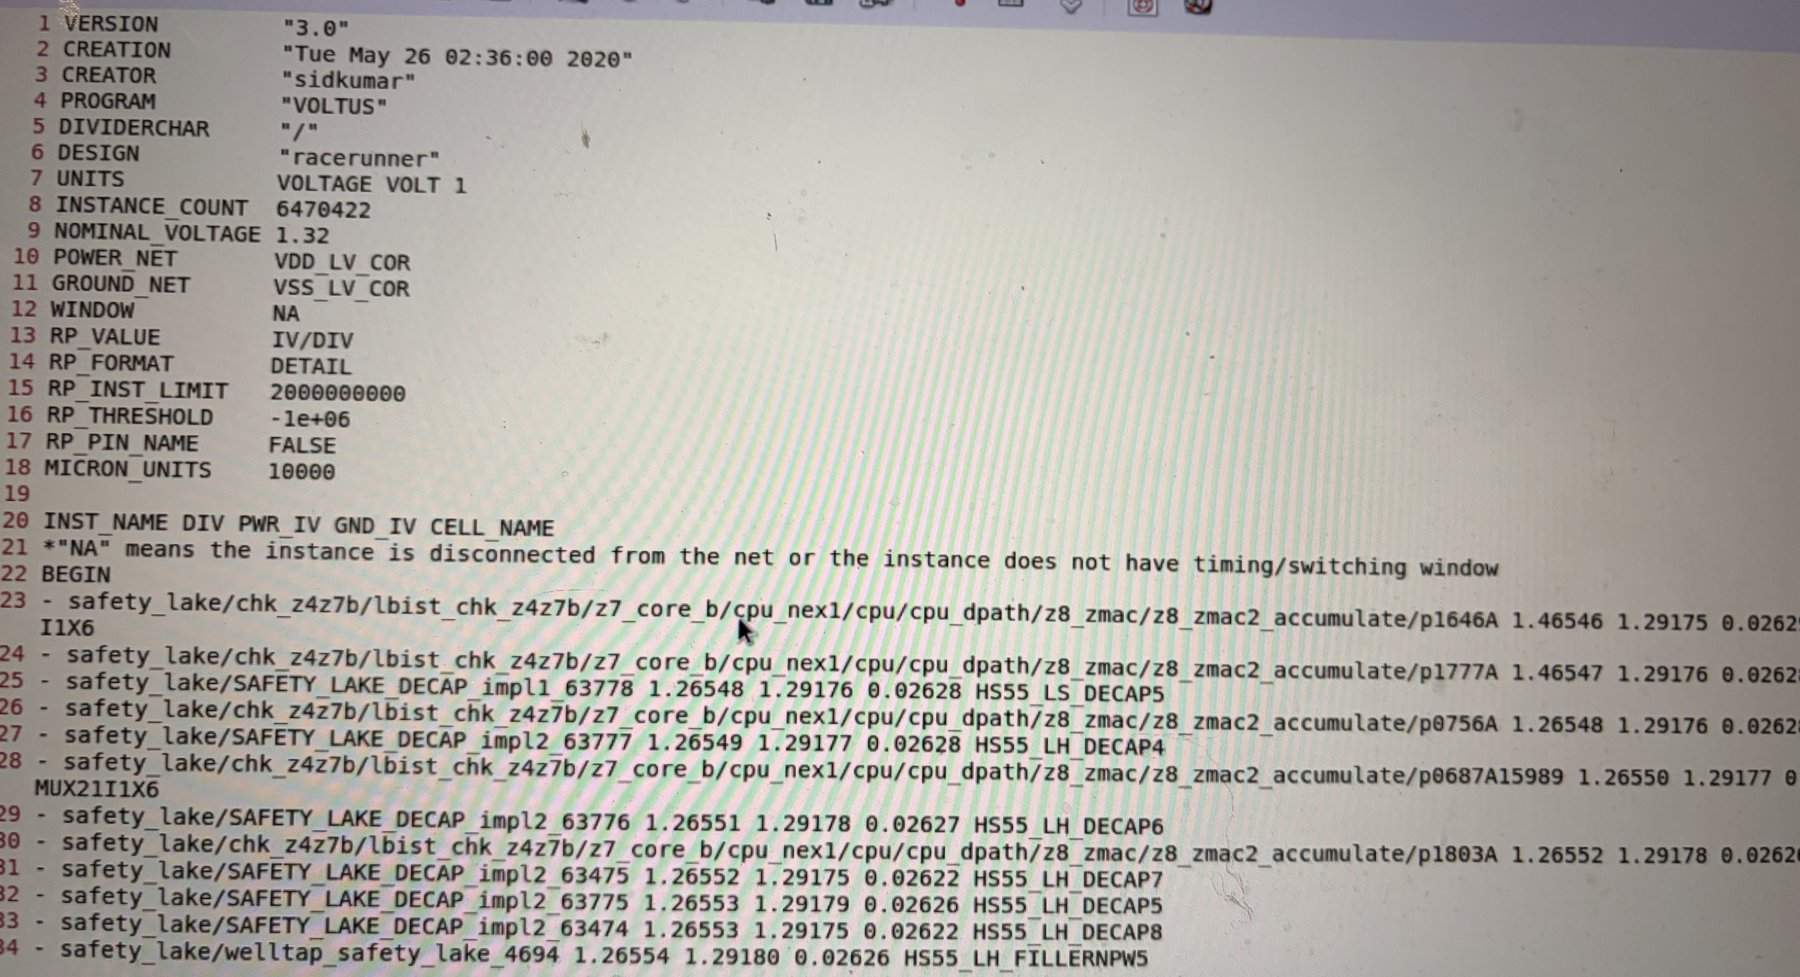
\includegraphics[width=\linewidth]{figures/photo_iv_file.jpg}
  \caption{\fn{.iv} IR report: header and per-instance DIV / PWR / GND voltages}
  \label{fig:iv}
\end{minipage}\hfill
\begin{minipage}[t]{0.4\linewidth}
  \centering
  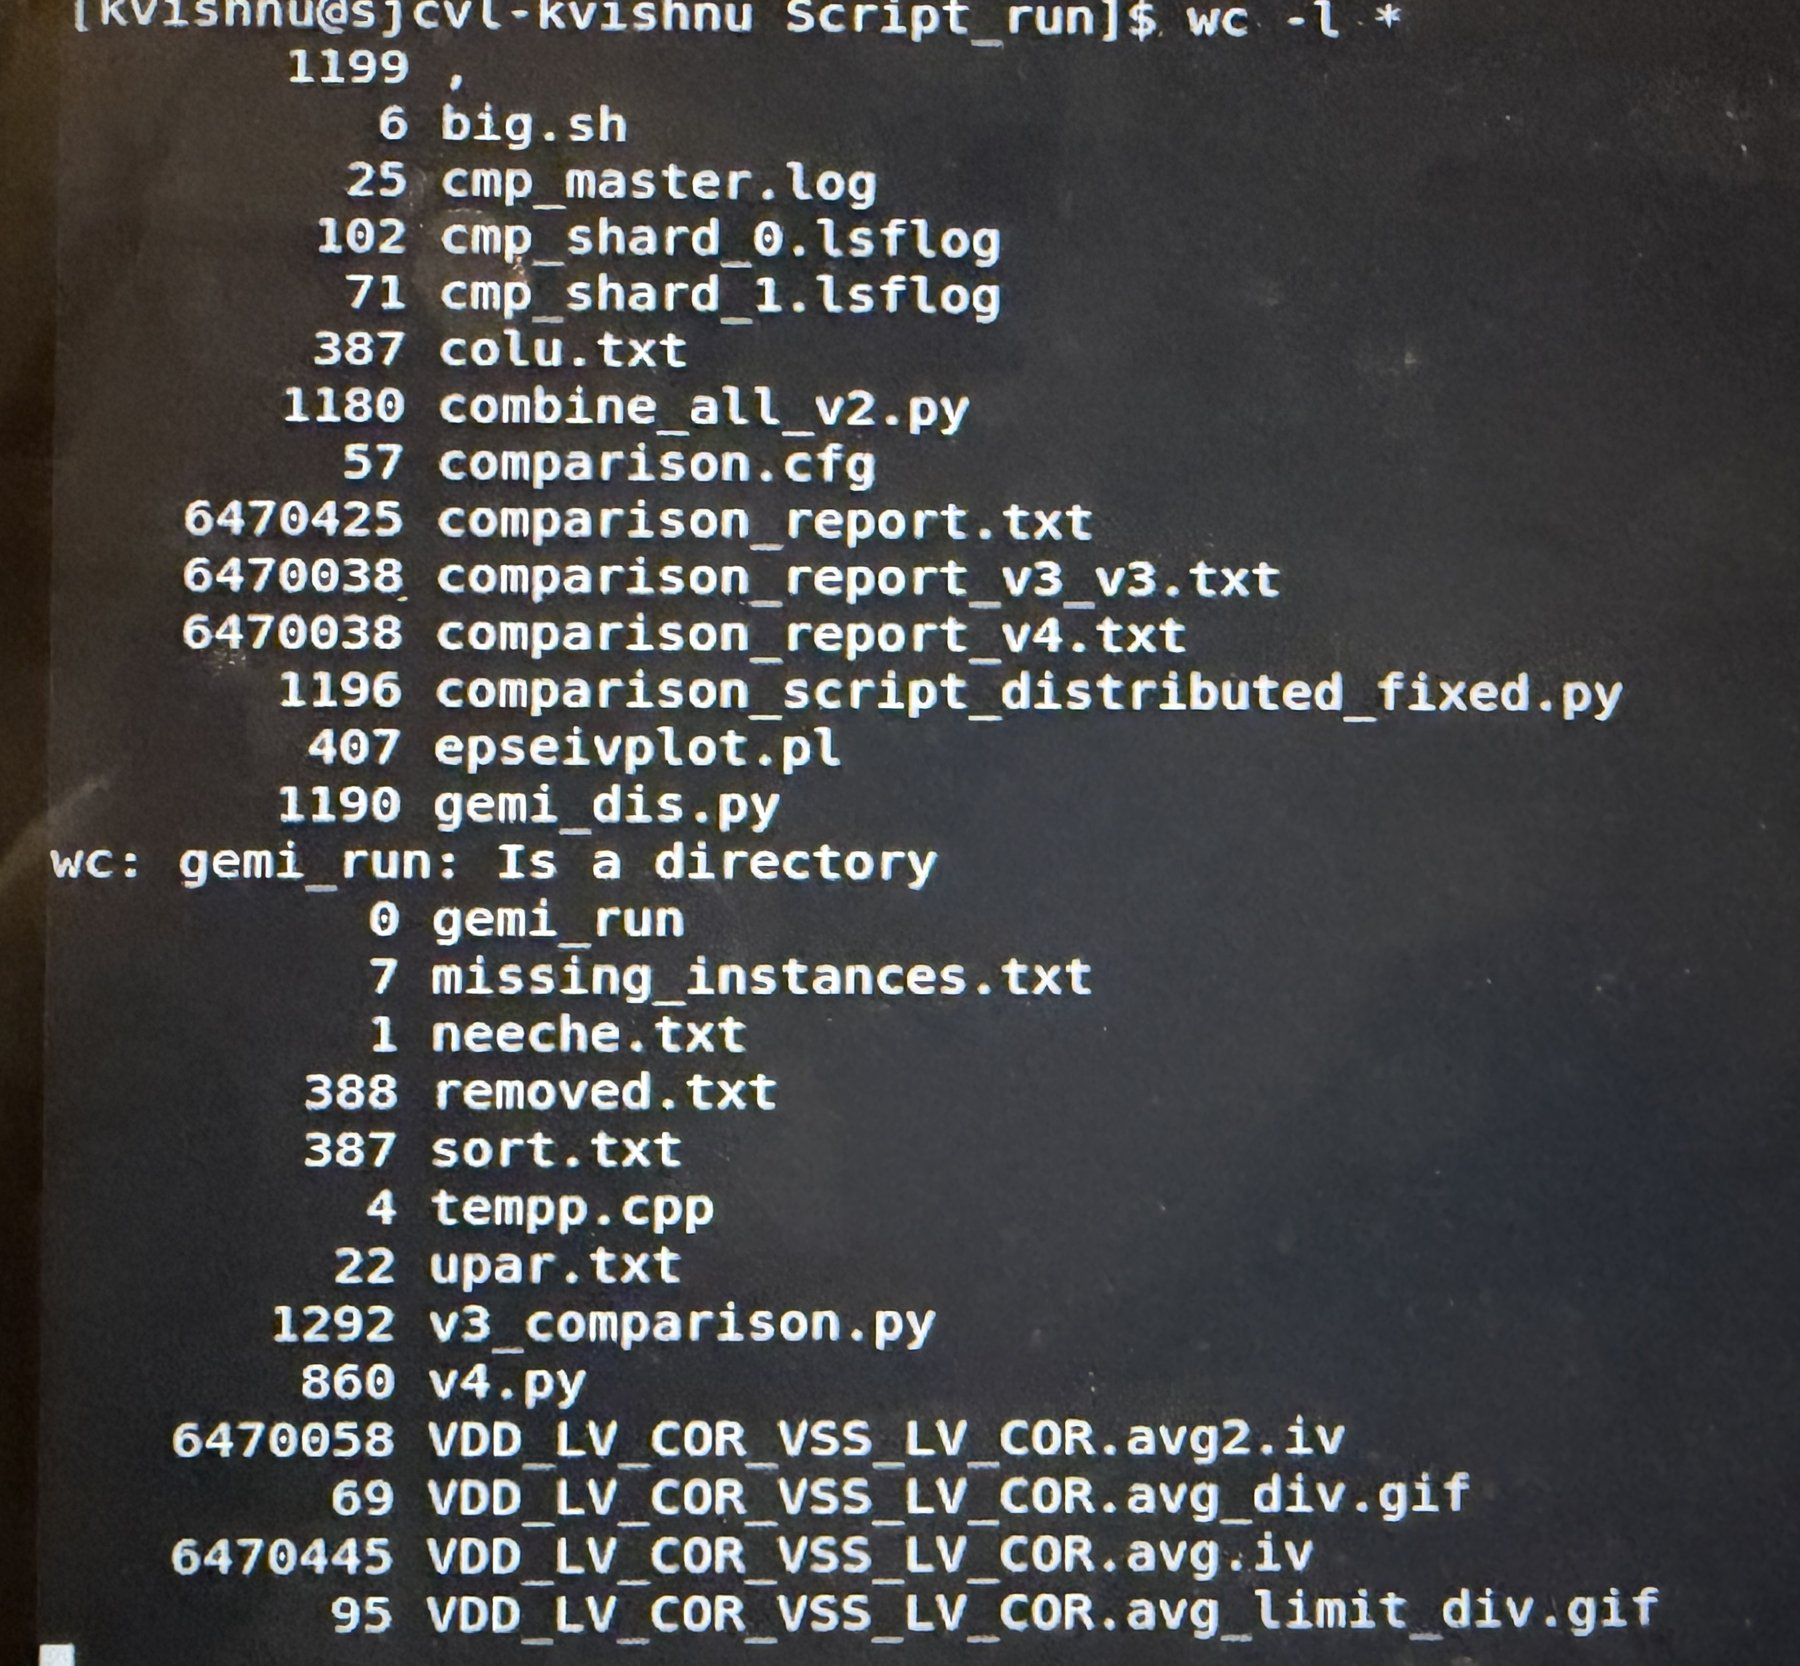
\includegraphics[width=\linewidth]{figures/photo_report_size.jpg}
  \caption{Scale: input \fn{.iv} files and comparison reports of $\approx$6.47\,M lines}
  \label{fig:size}
\end{minipage}
\end{figure}

\textbf{QCOM deployment.} On the customer farm, job submission failed until the \fn{bsub}
command was rebuilt from the profile (queue, runtime limit, \fn{select}/\fn{rusage}/\fn{span}
resource string). After the fix, shards dispatched correctly and the outlier plots were
proven against the customer data.

% ------------------------------------------------------------------
\subsection{Voltus--Tempus--Innovus ECO Study}
Self-driven study during a gap in assigned work: fix IR hotspots physically and prove that
power improves without breaking timing.

\begin{figure}[H]
\centering
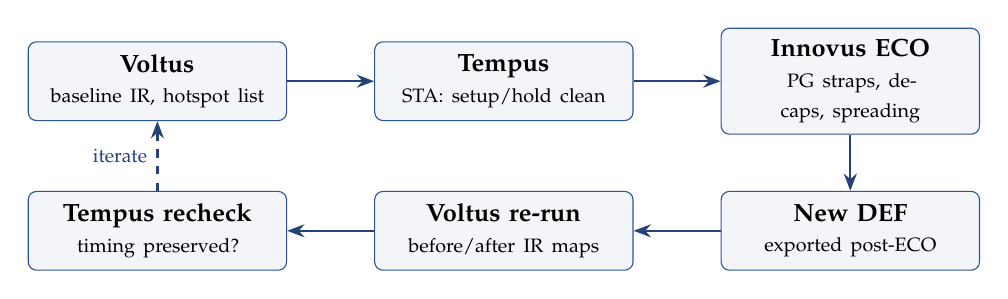
\begin{tikzpicture}[b/.style={box,text width=3.0cm}]
  \node[b] (v1) at (0,0)     {\textbf{Voltus}\\\scriptsize baseline IR, hotspot list};
  \node[b] (t1) at (4.4,0)   {\textbf{Tempus}\\\scriptsize STA: setup/hold clean};
  \node[b] (in) at (8.8,0)   {\textbf{Innovus ECO}\\\scriptsize PG straps, decaps, spreading};
  \node[b] (de) at (8.8,-1.9){\textbf{New DEF}\\\scriptsize exported post-ECO};
  \node[b] (v2) at (4.4,-1.9){\textbf{Voltus re-run}\\\scriptsize before/after IR maps};
  \node[b] (t2) at (0,-1.9)  {\textbf{Tempus recheck}\\\scriptsize timing preserved?};
  \draw[arr] (v1)--(t1); \draw[arr] (t1)--(in); \draw[arr] (in)--(de);
  \draw[arr] (de)--(v2); \draw[arr] (v2)--(t2);
  \draw[arr,dashed] (t2)--node[left,font=\scriptsize]{iterate} (v1);
\end{tikzpicture}
\caption{ECO loop: power fix in Innovus, verified by Voltus and Tempus}
\end{figure}

\begin{center}
\small
\begin{tabularx}{\linewidth}{@{}llX@{}}
\toprule
\textbf{Step} & \textbf{Tool} & \textbf{Purpose / result}\\
\midrule
Baseline      & Voltus  & IR-drop maps; instances with the worst effective voltage\\
Timing gate   & Tempus  & no setup/hold violations, so physical changes are safe to try\\
ECO           & Innovus & PG reinforcement, decap insertion, cell spreading near hotspots; new DEF\\
Re-analysis   & Voltus  & before/after comparison; localized hotspots reduced\\
Recheck       & Tempus  & confirm the ECO did not create timing violations\\
\bottomrule
\end{tabularx}
\end{center}

% ------------------------------------------------------------------
\subsection{Voltus Instance-Power Merge Bug}
\label{sec:bug}
While validating the combiner, instance power in Voltus' own top-level
\fn{power.instpwr.rpt.gz} did not match the per-partition report for the same run
(Voltus 25.13-s099\_1). The script was ruled out by reproducing the gap with Voltus outputs
alone:

\begin{figure}[H]
\centering
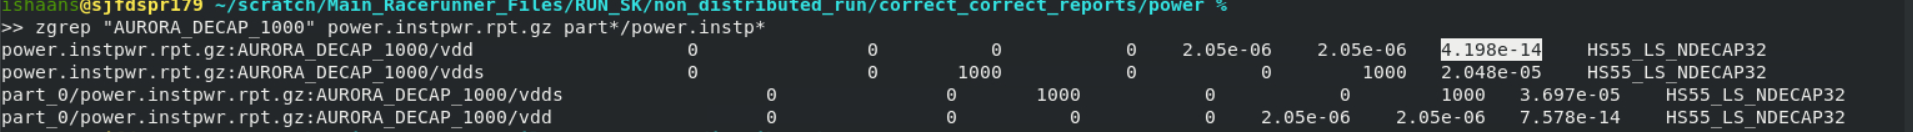
\includegraphics[width=\linewidth]{figures/voltus_bug.png}
\caption{\fn{zgrep} evidence: same instance, different power in top-level vs.\ \fn{part\_0} report}
\end{figure}

\begin{center}
\small
\begin{tabular}{@{}lcc@{}}
\toprule
\textbf{Instance / pin} & \textbf{\fn{part\_0} report} & \textbf{Top-level merged}\\
\midrule
\fn{AURORA\_DECAP\_1000/vdd}  & 7.578e-14 & 4.198e-14\\
\fn{AURORA\_DECAP\_1000/vdds} & 3.697e-05 & 2.048e-05\\
\bottomrule
\end{tabular}
\end{center}
Delivered to the tool team as a short deck with version, run script and a minimal
reproducible case.
\clearpage

% =========================== 7. CONCLUSION ===========================
\section{Conclusion}
Two months in Voltus Product Engineering took me from first static IR run to tools running on
a customer database. The core lesson: in signoff, speed matters only if the numbers are
provably right, so every tool shipped with logs, validation and a way to trace any output
back to raw data.

\subsection{Primary Objectives}
\begin{itemize}
  \item Cut Voltus post-processing time for distributed runs from hours to minutes.
  \item Automatically catch coverage gaps between Voltus instance data and switching data.
  \item Compare billion-row signoff reports and surface outliers visually.
  \item Understand the Voltus--Tempus--Innovus signoff/ECO loop hands-on.
\end{itemize}

\subsection{Implementation}
\begin{center}
\small
\begin{tabularx}{\linewidth}{@{}lXr@{}}
\toprule
\textbf{File} & \textbf{Responsibility} & \textbf{Lines}\\
\midrule
\fn{v3\_combine\_all\_reports.py}      & distributed combiner, all report types, C++ merge engine & 3236\\
\fn{combine.cfg}                       & grid/local switch, LSF profiles                         & 30\\
\fn{comparison\_script\_distributed.py} & sharded comparison, C++ merge-join, outlier plot        & 1773\\
\fn{comparison.cfg}                    & auto-local threshold, shard size, LSF profiles          & 42\\
cell-count script (Tcl + Python)       & instance dump, cell tally, switching-file match         & --\\
Review deck, usage guide, bug deck     & documentation and hand-over                             & --\\
\bottomrule
\end{tabularx}
\end{center}

\subsection{Challenges Faced}
\begin{itemize}
  \item \textbf{Distributed rail analysis:} failed on LSF but passed locally; power stage had
        to be separated from rail stage to isolate the fault.
  \item \textbf{Changing report formats:} a new run config broke parsing; fixed by
        format-tolerant parsing and re-testing on every run.
  \item \textbf{Memory:} multi-GB missing-instance JSON caused OOM when loaded whole; replaced
        by a streaming, disk-backed merge.
  \item \textbf{Merge-join desync:} an early C++ merge re-read an already-consumed line and
        reported false ``missing'' instances; fixed by caching the parsed key/value per side.
  \item \textbf{Customer farm:} \fn{bsub} resource strings that worked internally failed on
        QCOM; rebuilt from config profiles.
  \item \textbf{Trust in the reference:} Voltus' own merged report was itself inconsistent;
        proved with a minimal case before blaming or fixing the script.
\end{itemize}

\subsection{Outcomes}
\begin{itemize}
  \item Report merge: \textbf{3\,min 17\,s} for 115 file types / 1.95\,GB vs.\ up to
        $\sim$1\,h sequential.
  \item Comparison utility deployed and proven on the QCOM database, with outlier plots.
  \item Cell-count / DSP cross-check reading and dumping millions of lines in seconds.
  \item One Voltus data-integrity bug reported to R\&D with a reproducible case.
  \item Review deck, usage guide and full hand-over of code and configs.
\end{itemize}

\subsection{Limitations and Future Scope}
\begin{itemize}
  \item Extra readability column in the cell-count report pending specification.
  \item ECO study is qualitative; next step is a quantified before/after table
        (worst IR, hotspot count, WNS/TNS).
  \item Add a regression suite (golden merged reports) so every change is auto-validated.
  \item Interactive (Plotly/HTML) outlier view for drill-down on large runs.
  \item Upstream the combiner logic into the native Voltus merge step.
\end{itemize}

% =========================== 8. ENDING NOTE ==========================
\section{Ending Note}
This training bridged classroom physics ($P=\alpha CV^2f$, $V=IR$) and industrial signoff,
where those equations run on six million instances across a compute farm. I learned to build
tools for scale, to validate before claiming, and to report problems with evidence. AI
assistants made me faster, but understanding, testing and final decisions stayed with me.

I thank the Voltus Product Engineering team at Cadence and Delhi Technological University for
the opportunity. And yes, the pool table got a lot of use.

% ========================= 9. REFERENCES USED ========================
\section{References Used}
\begin{itemize}
  \item Cadence Design Systems : \url{https://www.cadence.com}
  \item Cadence Voltus, Tempus and Innovus user guides (internal documentation, release 25.1)
  \item IBM Spectrum LSF documentation : \url{https://www.ibm.com/docs/en/spectrum-lsf}
  \item Python \fn{concurrent.futures} : \url{https://docs.python.org/3/library/concurrent.futures.html}
  \item Python \fn{mmap} : \url{https://docs.python.org/3/library/mmap.html}
  \item GNU \fn{sort} : \url{https://www.gnu.org/software/coreutils/manual/html_node/sort-invocation.html}
  \item Matplotlib : \url{https://matplotlib.org}
  \item J.~M.~Rabaey, A.~Chandrakasan, B.~Nikoli\'c, \textit{Digital Integrated Circuits}, 2nd ed., Pearson.
  \item Claude (Anthropic) : \url{https://claude.ai}
  \item Gemini (Google) : \url{https://gemini.google.com}
\end{itemize}

\end{document}
